\input{preamble.tex}

\begin{document}
	
	\begin{titlepage}
	\newpage
	\begin{center}
		\includegraphics[width=\textwidth]{tit.png}
		Институт информационных и вычислительных технологий \\
			Кафедра управления и интеллектуальных технологий
		\vspace{1.25cm}
	\end{center}
	
	\vspace{1.2em}
	
	\begin{center}
		%\textsc{\textbf{}}
		\begin{spacing}{1}
			{\Large Отчёт по лабораторной работе \linebreak
			По дисциплине <<Теория автоматического управления>> \\}
			\vspace{0.3em}
			\large{\bf<<Исследование динамики линейных систем методом фазовой плоскости>>}
		\end{spacing}
	\end{center}
	
	\vspace{5em}
	

	\vspace{6em}
	
		\noindent Выполнили студенты: Михайловский М., Томчук В. \\
		Группа: А-03-21 \\
		Бригада: 1\\
		Проверил: Дементьев В.\,Ю.
	
	
	\vspace{\fill}
	
	\begin{center}
		Москва 2024
	\end{center}
	
\end{titlepage}
	\pagenumbering{arabic}
	\setcounter{page}{2}
	\tableofcontents
	\newpage
	
	\section{Постановка задачи}
	
	Дана нелинейная система автоматического управления (НСАУ), представленная на рис. \ref{scheme} с  нелинейным элементом (НЭ) типа трёхпозиционное реле с гистерезисом. Построить фазовый портрет системы, проанализировать переходные процессы для различных начальных условий (НУ), исследовать динамические свойства системы.
	
	Исследовать условия возникновения устойчивого предельного цикла в НСАУ при отсутствии в системе обратной связи по скорости в зависимости от ширины петли гистерезиса $l = \dfrac{m}{e}$. Экспериментально определить предельное значение $l$, при котором в системе наблюдается предельный цикл.
	
	\noindent{
		\begin{minipage}{.55\textwidth}
			\centering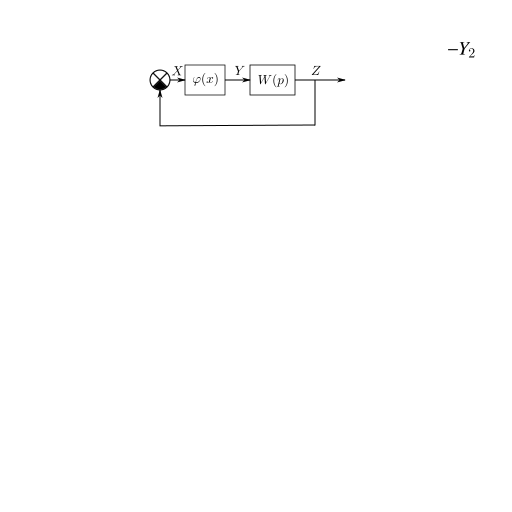
\includegraphics[width=\textwidth]{png/Схема.png}
			а)
		\end{minipage}
		\begin{minipage}{.45\textwidth}
			\centering\includegraphics[width=.65\textwidth]{png/НЭ.png}
			
			б)
		\end{minipage}
		\captionof{figure}{а) Структурная схема НСАУ; б) Вид характеристики НЭ}
		\label{scheme}
	}


	Параметры звеньев:
	\begin{align*}
		& W_1(p) = K_1 = 10 \\
		& W_2(p) = \frac{K_2}{p} = \frac{1}{p} \\
		& W_3(p) = \frac{K_3}{1+pT_3} = \frac{5}{1+p} \\
		& W_4(p) = K_4 = 2
	\end{align*}
	
	Параметры НЭ:
	\begin{equation*}
		a = 0,2,\;e=5,0,\;m=2,5
	\end{equation*}


	\section{Подготовка к работе}
	\subsection{Получение уравнения системы и его решение}
	
	Запишем уравнения, задающиеся структурной схемой:
	\begin{equation*}
		\begin{cases}
			Y_1 = Y_2\cdot W_2(p) = \dfrac{Y_2}{p} \\
			Y_2 = -Z(U)\cdot W_3(p) = -\dfrac{5 Z(U)}{1+p} \\
			U = Y_1\cdot W_1(p) + Y_2 \cdot W_4(p) = 10Y_1 + 2Y_2
		\end{cases}
	\end{equation*}

	Переходя во временную область, получаем следующую систему в форме Коши:
	\begin{equation}
		\begin{cases}
			y'_1 = y_2 \\
			y'_2 = -y_2 - 5z(10y_1 + 2y_2)
		\end{cases}
		\label{coshi}
	\end{equation}
	\begin{equation*}
		z(10y_1+2y_2) = 
		\begin{cases}
			0,2, & 10y_1+2y_2 \geq 5 \\
			0,2, & 2,5 \leq 10y_1+2y_2 \leq 5,\;z^{-} = 0,2 \\
			0, & 2,5 \leq 10y_1+2y_2 \leq 5,\;z^{-} = 0 \\
			0 & -2,5 \leq 10y_1+2y_2 \leq -2,5\\
			0, & -5 \leq 10y_1+2y_2 \leq -2,5,\;z^{-} = 0 \\
			-0,2, & -5 \leq 10y_1+2y_2 \leq -2,5,\;z^{-} = -0,2 \\
			-0,2, & 10y_1+2y_2 \leq 5 \\
		\end{cases}
	\end{equation*}
	
	Полупрямые переключения:
	\begin{equation}
		\left[
		\begin{aligned}
			&10y_1 + 2y_2 = 5,\;y_2 \geq 0 \\
			&10y_1 + 2y_2 = 2,5,\;y_2 \leq 0 \\
			&10y_1 + 2y_2 = -2,5,\;y_2 \geq 0 \\
			&10y_1 + 2y_2 = -5,\;y_2 \leq 0 \\
		\end{aligned}\right.
		\label{lines}
	\end{equation}

	Учитывая то, какие значения может принимать $z(u)$, рассмотрим более общую систему. Случаи $B=-1,\, 0,\, 1$ соответствуют 3 областям имеющимся в исследуемой НСАУ:
	\begin{equation*}
		\begin{cases}
			y'_1 = y_2 \\
			y'_2 = -y_2 - B
		\end{cases}
	\end{equation*}

	Решим систему дифференциальных уравнений:
	\begin{equation*}
		\dv{y_2}{y_1}= -\frac{y_2+B}{y_2} \Rightarrow \int_{y_{2_0}}^{y_2} \frac{y_2}{y_2+B} \dd{y_2} = -\int_{y_{1_0}}^{y_1} \dd{y_1}
	\end{equation*}
	\begin{equation*}
		\int_{y_{2_0}}^{y_2} \frac{y_2}{y_2+B} \dd{y_2} = \int_{y_{2_0}}^{y_2} \left(1 -\frac{B}{y_2+B}\right) \dd{y_2} = y_2 - y_{2_0} - B\ln{\left|\frac{y_2+B}{y_{2_0}+B}\right|} = y_{1_0} - y_1 \Rightarrow
	\end{equation*}
	\begin{equation*}
		\Rightarrow -y_2 + B\ln{|y_2+B|} = y_1 + C,\;\text{где}\; C= y_{1_0} + y_{2_0} - B\ln{|y_{2_0} - B|}
	\end{equation*}

	\subsection{Построение фазового портрета} 
	
	Рассмотрим 3 области, задаваемые значениями реле:
	
	\underline{Область I}. $z(u) = 0,2,\;B=1$. Уравнение фазовых траекторий:
	\begin{equation*}
		-y_2 + \ln{|y_2+1|} = y_1 + C
	\end{equation*}

	Имеется асимптота $y_2 = -1$, в ней $y_1\xrightarrow[y_2\to-1]{} -\infty$

	\underline{Область II}. $z(u) = 0,\;B=0$. Уравнение фазовых траекторий:
	\begin{equation*}
		-y_2 = y_1 + C
	\end{equation*}
	Это уравнение семейства прямых.
	
	\underline{Область III}. $z(u) = -0,2,\;B=-1$. Уравнение фазовых траекторий:
	\begin{equation*}
		-y_2 - \ln{|y_2-1|} = y_1 + C
	\end{equation*}

	Имеется асимптота $y_2 = 1$, в ней $y_1\xrightarrow[y_2\to1]{} -\infty$.
	
	Итоговые фазовые портреты для всех областей представлены на рис. \ref{tr}.

	\noindent{
	\begin{minipage}{.333\textwidth}
		\centering\includegraphics[width=.95\textwidth]{png/зона1.png}
		I~область
	\end{minipage}	
	\begin{minipage}{.333\textwidth}
		\centering\includegraphics[width=.95\textwidth]{png/зона2.png}
		II~область
	\end{minipage}	
	\begin{minipage}{.333\textwidth}
		\centering\includegraphics[width=.95\textwidth]{png/зона3.png}
		III~область
	\end{minipage}

	\captionof{figure}{Фазовые портреты для 3 областей}
	\label{tr}
}

	Теперь исследованы все необходимые параметры для построения фазового портрета системы. Построенный общий фазовый портрет представлен на рис. \ref{FP}. 
	
	Как видим, в данной системе отсутствуют такие особые режимы как устойчивый предельный цикл или скользящий режим. Однако, при малой ширине петли гистерезиса или меньшей зоне нечувствительности НЭ могут возникнуть автоколебания.	
	
	\begin{figure}[h]
		\centering\includegraphics[width=.8\textwidth]{png/FP.png}
		\caption{Фазовый портрет НСАУ}
		\label{FP}
	\end{figure}

	\section{Выполнение работы}
	\subsection{Моделирование фазового портрета}
	
	Рассмотрим виды фазовых траекторий в основных областях. Для их построения заданы параметры, представленные на рис. \ref{params_m}. Для первой области имеем нелинейные портреты рис. \ref{obl1}, \ref{obl1p}. Как видим, траектории имеют асимптоту при $y=-1$.
	
	\begin{figure}[h]
		\centering\includegraphics[width=.4\textwidth]{png/10.png}
		\caption{Параметры для моделирования 3 областей}
		\label{params_m}
	\end{figure}
	
	Для третьей области фазовый портрет похожий, и имеет следующий вид: рис. \ref{obl3}, \ref{obl3p}. Они симметричны I области и имеют асимптоту при $y=1$.
	
	\begin{figure}[h]
		\centering\includegraphics[width=.55\textwidth]{png/1.png}
		\caption{Фазовый портрет для I области}
		\label{obl1}
	\end{figure}

	\noindent{
	\begin{minipage}{.5\textwidth}
		\centering\includegraphics[width=\textwidth]{png/2.png}
	\end{minipage}	
	\begin{minipage}{.5\textwidth}
		\centering\includegraphics[width=\textwidth]{png/3.png}
	\end{minipage}

	\captionof{figure}{Переходные процессы для I области}
	\label{obl1p}
}
	\begin{figure}[h]
		\centering\includegraphics[width=.55\textwidth]{png/6.png}
		\caption{Фазовый портрет для III области}
		\label{obl3}
	\end{figure}
	
	\noindent{
		\begin{minipage}{.5\textwidth}
			\centering\includegraphics[width=\textwidth]{png/7.png}
		\end{minipage}	
		\begin{minipage}{.5\textwidth}
			\centering\includegraphics[width=\textwidth]{png/8.png}
		\end{minipage}

	\captionof{figure}{Переходные процессы для III области}
	\label{obl3p}
}

	Для второй области фазовые траектории имеют линейный вид: рис. \ref{obl2}.

	\vspace{0.5em}

	\noindent{
		\begin{minipage}{.45\textwidth}
			\centering\includegraphics[height=8em]{png/4.png}
		\end{minipage}	
		\begin{minipage}{.5\textwidth}
			\centering\includegraphics[height=8em]{png/5.png}
		\end{minipage}
		
		\captionof{figure}{Фазовый портрет и переходные процессы для II области}
		\label{obl2}
	}

	Приведём уравнения полупрямых (\ref{lines}) к следующему виду:
	\begin{equation*}
		\left[
		\begin{aligned}
			&y_1 = 0,5 - 0,2y_2,\;&y_2 \geq 0 \\
			&y_1 = 0,25 - 0,2y_2,\;&y_2 \leq 0 \\
			&y_1 = -0,25 - 0,2y_2,\;&y_2 \geq 0 \\
			&y_1 = -0,5 - 0,2y_2,\;&y_2 \leq 0 \\
		\end{aligned}\right.
	\end{equation*}

	Эти параметры были указаны при построении рис. \ref{lines_p}.
	
	\begin{figure}[h]
		\centering\includegraphics[width=.4\textwidth]{png/9.png}
		\caption{Заданные уравнения полупрямых для моделирования}
		\label{lines_p}
	\end{figure}

	В результате получаем следующий фазовый портрет НСАУ: рис. \ref{NSAU_portret}.
	
	\begin{figure}[h]
		\centering\includegraphics[width=.7\textwidth]{png/11.png}
		\caption{Фазовый портрет исследуемой НСАУ}
		\label{NSAU_portret}
	\end{figure}
	
	Фазовый портрет имеет характер, подобный тому, который был получен в подготовке. Видно, что в системе не наблюдается особых динамических режимов, таких как скользящий режим или автоколебания.
	
	Переходные процессы имеют следующий вид: рис. \ref{nsau_p}.
	
	\noindent{
		\begin{minipage}{.5\textwidth}
			\centering\includegraphics[width=\textwidth]{png/12.png}
		\end{minipage}	
		\begin{minipage}{.5\textwidth}
			\centering\includegraphics[width=\textwidth]{png/13.png}
		\end{minipage}
		
		\captionof{figure}{Фазовый портрет и переходные процессы для II области}
		\label{nsau_p}
	}

	\subsection[Влияние ширины петли гистерезиса на автоколебания]{Исследования влияния ширины петли гистерезиса на наличие автоколебаний}
	
	Будем изменять левую или правую границу переключения реле для определения предельной ширины гистерезиса, при которой появляются автоколебания. В данном эксперименте исследуем систему без обратной связи по скорости, то есть $K_4 = 0 \Rightarrow W_4(p)=0$, рис. \ref{scheme2}. Это повлияет на наклон прямых переключения -- они будут вертикальными.
	
	\begin{figure}[h]
		\centering\includegraphics[width=.6\textwidth]{png/схема2.png}
		\caption{Схема для исследования}
		\label{scheme2}
	\end{figure}

	\begin{figure}[h]
		\centering\includegraphics[width=.6\textwidth]{png/15.png}
		\caption{Фазовый портрет для широкой петли гистерезиса: $e=2,5$}
		\label{issl1}
	\end{figure}
	
	Чем шире петля гистерезиса, тем дальше система от того, чтобы оказаться в режиме автоколебаний, рис. \ref{issl1}. Это значит, что автоколебания могут возникнуть при узкой петле гистерезиса.
	
	Для данной системы автоколебания возникнут только при более малых значениях $m$ и $e$, чем данные в постановке задачи. Возьмём следующие меньшие значения: $m=0,1,\,e=0,25$. При таких параметрах наблюдаются автоколебания: рис. \ref{issl2}, \ref{issl2_p}.
	
	\begin{figure}[h]
		\centering\includegraphics[width=.6\textwidth]{png/19.png}
		\caption{Фазовый портрет c автоколебаниями, $m=0,1,\,e=0,25$}
		\label{issl2}
	\end{figure}

	\begin{figure}[h]
		\centering\includegraphics[width=.6\textwidth]{png/20.png}
		\caption{Переходной процесс c автоколебаниями, $m=0,1,\,e=0,25$}
		\label{issl2_p}
	\end{figure}

	Предельные параметры, при которых имеются автоколебания: $m_\text{пр} = 0,13,\,e_\text{пр}=0,25$: рис. \ref{issl3}.
	
	\begin{figure}[h]
		\centering\includegraphics[width=.6\textwidth]{png/16.png}
		\caption{Фазовый портрет при $m_\text{пр} = 0,13,\,e_\text{пр}=0,25$}
		\label{issl3}
	\end{figure}
	
	При увеличении $m$ автоколебания пропадают: рис. \ref{issl4}, \ref{issl4_p}. Итого получаем следующую предельную ширину гистерезиса: 
	
	\begin{equation*}
		l_\text{пр} = \dfrac{m_\text{пр}}{e_\text{пр}} = \dfrac{0,13}{0,25} = 0,52
	\end{equation*}

	\begin{figure}[h]
		\centering\includegraphics[width=.6\textwidth]{png/17.png}
		\caption{Фазовый портрет, $m=0,18,\,e=0,25$}
		\label{issl4}
	\end{figure}
	
	\begin{figure}[h]
		\centering\includegraphics[width=.6\textwidth]{png/18.png}
		\caption{Переходной процесс, $m=0,18,\,e=0,25$}
		\label{issl4_p}
	\end{figure}
	
	\clearpage
	
	\section{Выводы}
	
	Была исследована нелинейная система автоматического управления с трёхпозиционным реле с гистерезисом. Её динамика была рассмотрена с помощью метода фазовой плоскости, а затем исследование динамики было повторено с помощью компьютерного моделирования.
	
	Изначальная система оказалась устойчивой и не имела особых динамических режимов, таких как скользящий режим или автоколебания.
	
	С помощью компьютерного моделирования в аналогичной системе без обратной связи по скорости было исследовано влияние ширины петли гистерезиса на наличие предельного цикла. Автоколебания в такой системе наблюдаются только для малых значений параметров $m,\,e$ реле. При их больших значениях такого режима в системе не наблюдается. 
	
	Предельным значением ширины петли гистерезиса, при котором есть автоколебания оказалось значение $l_\text{пр} = 0,52$. 
	
\end{document}
